\documentclass[11pt]{report}
\usepackage{tikz}
\usepackage{amsmath}
\usepackage{placeins}
\usepackage{booktabs}
\usetikzlibrary{fit,positioning}
\setcounter{chapter}{9}
\begin{document}
\chapter{Problems}
\section{}
\textit{The joint probability model between variables $\{x_i\}_{i=1}^7$ factorizes as}
\begin{equation} 
\begin{aligned}
&Pr(x_1, x_2, x_3, x_4, x_5, x_6, x_7) = \\
&\quad \quad Pr(x_1) Pr(x_3) Pr(x_7) Pr(x_2 | x_1, x_3) Pr(x_5 | x_7, x_2) Pr(x_4 | x_2) Pr (x_6 | x_5, x_4) \notag
\end{aligned}
\end{equation}
\textit{Draw a directed graphical model relating these variables. Which variables form the Markov blanket of variable $x_2$?}
\begin{figure}[h]
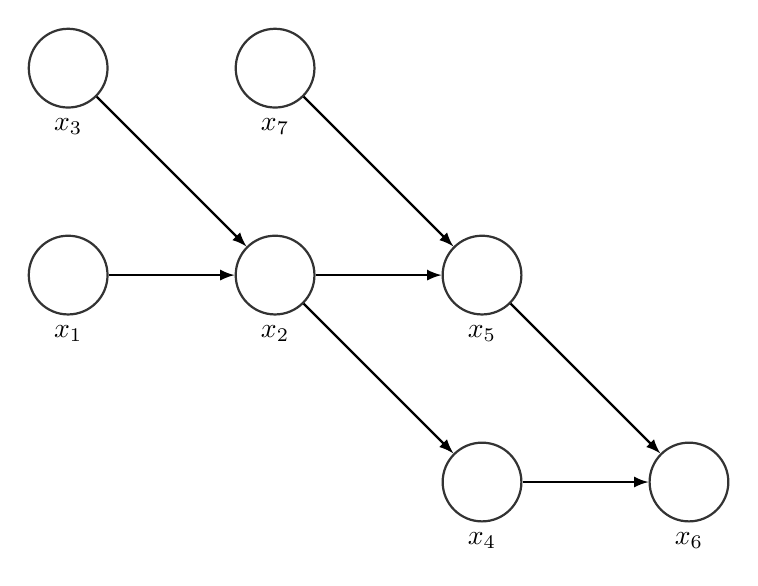
\begin{tikzpicture}
\tikzstyle{main}=[circle, minimum size = 10mm, thick, draw =black!80, node distance = 16mm]
\tikzstyle{connect}=[-latex, thick]
\tikzstyle{box}=[rectangle, draw=black!100]
  \node[main, fill = white!100] (x1) [label=below:$x_1$] { };
  \node[main] (x2) [right=of x1,label=below:$x_2$] { };
  \node[main] (x3) [above=of x1,label=below:$x_3$] {};
  \node[main] (x5) [right=of x2,label=below:$x_5$] { };
  \node[main] (x4) [below=of x5,label=below:$x_4$] { };
  \node[main] (x6) [right=of x4,label=below:$x_6$] { };
  \node[main] (x7) [above=of x2,label=below:$x_7$] { };
  \path (x1) edge [connect] (x2)
           (x3) edge [connect] (x2)
           (x2) edge [connect] (x5)
           (x7) edge [connect] (x5)
           (x2) edge [connect] (x4)
           (x5) edge [connect] (x6)
           (x4) edge [connect] (x6);
\end{tikzpicture}
\end{figure}

The Markov blanket of $x_2$ is $\{x_1, x_3, x_5, x_7 \}$ (the parents, children and co-parents of the children of $x_2$).
\FloatBarrier

\section{}
\textit{Write out the factorization corresponding to the directed graphical model in Figure 10.14a }
\begin{equation} 
\begin{aligned}
Pr(x_1, ..., x_{15}) = &Pr(x_1) Pr(x_2) Pr(x_3) Pr(x_4 | x_1, x_2) Pr(x_5 | x_2, x_3) Pr(x_6) Pr(x_7) Pr(x_8 | x_4, x_5) \\
    & Pr(x_9 | x_3, x_5, x_6) Pr(x_{10} | x_7) Pr(x_{11} | x_8, x_{10}) Pr(x_{12} | x_8, x_9) Pr(x_{13} | x_9) \\
    & Pr(x_{14} | x_{11}) Pr(x_{15} | x_{12}) \notag
\end{aligned} 
\end{equation}

\section{}
\textit{An undirected graphical model has the form}

\begin{equation} 
\begin{aligned}
Pr(x_1, ..., x_{6}) = & \frac{1}{Z} \phi_1[x_1, x_2, x_5] \phi_2[x_2, x_3, x_4] \phi_3[x_1, x_5] \phi_4[x_5, x_6] \notag
\end{aligned} 
\end{equation}

\textit{Draw the undirected graphical model that corresponds to this factorization.}

\begin{figure}[h]
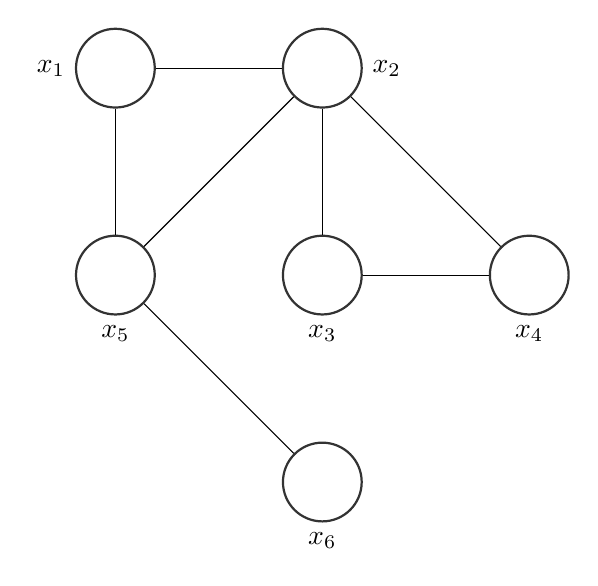
\begin{tikzpicture}
\tikzstyle{main}=[circle, minimum size = 10mm, thick, draw =black!80, node distance = 16mm]
\tikzstyle{connect}=[-latex, thick]
\tikzstyle{box}=[rectangle, draw=black!100]
  \node[main, fill = white!100] (x1) [label=left:$x_1$] { };
  \node[main] (x2) [right=of x1,label=right:$x_2$] { };
  \node[main] (x3) [below=of x2,label=below:$x_3$] {};
  \node[main] (x5) [below=of x1,label=below:$x_5$] { };
  \node[main] (x4) [right=of x3,label=below:$x_4$] { };
  \node[main] (x6) [below=of x3,label=below:$x_6$] { };
  \path (x1) edge (x2)
           (x1) edge (x5)
           (x2) edge (x5)
           (x2) edge (x3)
           (x2) edge (x4)
           (x3) edge (x4)
           (x5) edge (x6)
           ;
\end{tikzpicture}
\end{figure}

\section{}
\textit{Write out the factorization corresponding to the undirected graphical model in Figure 10.14b.}
\begin{equation} 
\begin{aligned}
Pr(x_1, ..., x_{15}) = \frac{1}{Z} &\phi_1[x_3] \phi_2[x_1, x_4] \phi_3[x_2, x_4, x_8] \phi_4[x_2, x_5, x_8] \phi_5[x_5, x_9] \\
  & \phi_6[x_6, x_9] \phi_7[x_8, x_{12}] \phi_8[x_9, x_{12}, x_{13}, x_{15}] \phi_9[x_8, x_{11}] \phi_{10}[x_7, x_{10}] \\
  & \phi_{11}[x_7, x_11] \phi_{12}[x_{11}, x_{14}] \notag
\end{aligned} 
\end{equation}
\FloatBarrier

\section{}
\textit{Consider the undirected graphical model defined over binary values $\{x_i\}_{i=1}^4 \in \{0, 1\}$ defined by }
\begin{equation} 
\begin{aligned}
Pr(x_1, x_2, x_3, x_4) = & \frac{1}{Z} \phi(x_1, x_2) \phi(x_2, x_3) \phi(x_3, x_4) \phi(x_4, x_1) \text{,} \notag
\end{aligned} 
\end{equation}
\textit{where the function $\phi$ is defined by}
\begin{equation} 
\begin{aligned}
&\phi(0,0) = 1 \quad \quad & \phi(1,1) = 2 \\
&\phi(0,1) = 0.1 \quad \quad &\phi(1,0) = 0.1 \notag
\end{aligned} 
\end{equation}
\textit{ Compute the probability of each of the 16 possible states of this system.}

\begin{table}[h]
\begin{tabular}{c c c c|c c c c r r}
\toprule
 $x_1$ & $x_2$ & $x_3$ & $x_4$  & $\phi(x_1, x_2)$ & $\phi(x_2, x_3)$ & $\phi(x_3, x_4)$ & $\phi(x_4, x_1)$ &
       $Z Pr(...)$ & $Pr(...)$ \\ \midrule
 0 & 0 & 0 & 0 & 1. & 1. & 1. & 1. & 1.0000 & .057870 \\
 0 & 0 & 0 & 1 & 1. & 1. & 0.1& 0.1 & 0.0100 & .000579 \\
 0 & 0 & 1 & 0 & 1. & 0.1 & 0.1  & 1. & 0.0100 & .000579 \\
 0 & 0 & 1 & 1 & 1. & 0.1 & 2. & 0.1 & 0.0200 & .001157 \\
 0 & 1 & 0 & 0 & 0.1 & 0.1  & 1. & 1.& 0.0100 & .000579 \\
 0 & 1 & 0 & 1 & 0.1 & 0.1 & 0.1 & 0.1 & 0.0001 & .000006 \\
 0 & 1 & 1 & 0 & 0.1 & 2. & 0.1 & 1. & 0.0200 & .001157 \\
 0 & 1 & 1 & 1 & 0.1 & 2. & 2. & 0.1 & 0.0400 & .002315 \\
 1 & 0 & 0 & 0 & 0.1 & 1. & 1. &  0.1 & 0.0100 & .000579 \\
 1 & 0 & 0 & 1 & 0.1 & 1. & 0.1 & 2. & 0.0200 & .001157 \\
 1 & 0 & 1 & 0 & 0.1 & 0.1 & 0.1 & 0.1 & 0.0001 & .000006 \\
 1 & 0 & 1 & 1 & 0.1 & 0.1 & 2. & 2. & 0.0400 & .002315 \\
 1 & 1 & 0 & 0 & 2.& 0.1 & 1. & 0.1 & 0.0200 & .001157 \\
 1 & 1 & 0 & 1 & 2. & 0.1 & 0.1 & 2. & 0.0400 & .002315 \\
 1 & 1 & 1 & 0 & 2. & 2. & 0.1 & 0.1 & 0.0400 & .002315 \\
 1 & 1 & 1 & 1 & 2. & 2. & 2. & 2. & 16.0000 & .925914 \\ \midrule
 & & & & & & & & 17.2802 & 1.000000 \\ \bottomrule
\end{tabular}
\end{table}
\FloatBarrier 

We can attempt to check this by sampling from the distribution e.g. using Gibbs sampling. To do this we need the conditional probability distribution for each $x_i$. By symmetry we just need to calculate the conditional distribution for $x_1$.

\begin{align*}
  Pr(x_1 | x_{\backslash 1}) &= \frac{Pr(x_1, x_2, x_3, x_4)}{\sum_{x_1} Pr(x_1, x_2, x_3, x_4)} \\
     &= \frac{\frac{1}{Z} \phi(x_1, x_2) \phi(x_2, x_3) \phi(x_3, x_4) \phi(x_4, x_1)}
         {\sum_{x_1}  \frac{1}{Z} \phi(x_1, x_2) \phi(x_2, x_3) \phi(x_3, x_4) \phi(x_4, x_1)} \\
     &= \frac{\phi(x_1, x_2) \phi(x_2, x_3) \phi(x_3, x_4) \phi(x_4, x_1)}
     	{\phi(x_2, x_3) \phi(x_3, x_4) \sum_{x_1} \phi(x_1, x_2) \phi(x_4, x_1)} \\
     &= \frac {\phi(x_1, x_2) \phi(x_4, x_1)}{\sum_{x_1} \phi(x_1, x_2) \phi(x_4, x_1)} \\
 \end{align*}
 \begin{align*}
  Pr(x_1 = 0 | x_2 = 0, x_4 = 0) &= \frac{1. \times 1.}{1. \times 1. + 0.1 \times 0.1} = \frac{1.}{1.01} = 0.9901 \\
  Pr(x_1 = 1 | x_2 = 0, x_4 = 0) &= 1 - Pr(x_1 = 0 | x_2 = 0, x_4 = 0) = 1 - 0.9901 = 0.0099 \\
  Pr(x_1 = 0 | x_2 = 0, x_4 = 1) &= \frac{1. \times 0.1}{1. \times 0.1 + 0.1 \times 2.} = \frac{0.1}{0.3} = 0.3333 \\
  Pr(x_1 = 1 | x_2 = 0, x_4 = 1) &= 1 - Pr(x_1 = 0 | x_2 = 0, x_4 = 0) = 1 - 0.3333 = 0.6667 \\
  Pr(x_1 = 0 | x_2 = 1, x_4 = 0) &= \frac{0.1 \times 1.}{0.1 \times 1. + 2. \times 0.1} = \frac{0.1}{0.3} = 0.3333 \\
  Pr(x_1 = 1 | x_2 = 1, x_4 = 0) &= 1 - Pr(x_1 = 0 | x_2 = 0, x_4 = 0) = 1 - 0.3333 = 0.6667 \\
  Pr(x_1 = 0 | x_2 = 1, x_4 = 1) &= \frac{0.1 \times 0.1}{0.1 \times 0.1 + 2. \times 2.} = \frac{0.01}{4.01} = 0.0025 \\
  Pr(x_1 = 1 | x_2 = 1, x_4 = 1) &= 1 - Pr(x_1 = 0 | x_2 = 0, x_4 = 0) = 1 - 0.0025 = 0.9975 \\
\end{align*}



\end{document}